\documentclass[12pt]{article}
\usepackage[utf8]{inputenc}
\usepackage{geometry}
\geometry{letterpaper, margin=1in}
\usepackage{amsmath}
\usepackage{graphicx} % For embedding images (Q1b)
\usepackage{enumitem}
\usepackage{booktabs} % For nice tables
\usepackage{tikz}

\title{CS 412 Assignment 5 Report}
\author{Donggyu Park}
\date{\today}

\begin{document}

\maketitle

% ==========================================
% Question 1
% ==========================================
\section*{1. Frequent Pattern Mining (25 points)}

\begin{enumerate}[label=(\alph*)]
    \item
    % TODO: Show Apriori algorithm steps here.
    Given $minsup = 2$:

    \textbf{Scan 1:} Count the support of each 1-itemset.
    \begin{center}
    \begin{tabular}{|c|c|}
        \hline
        \textbf{Itemset} & \textbf{Support} \\ \hline
        \{V\} & 1 \\ \hline
        \{W\} & 5 \\ \hline
        \{X\} & 6 \\ \hline
        \{Y\} & 6 \\ \hline
        \{Z\} & 7 \\ \hline
    \end{tabular}
    \end{center}
    Filter out itemsets with support $< 2$.
    \begin{center}
    \begin{tabular}{|c|c|}
        \hline
        \textbf{Itemset ($L_1$)} & \textbf{Support} \\ \hline
        \{W\} & 5 \\ \hline
        \{X\} & 6 \\ \hline
        \{Y\} & 6 \\ \hline
        \{Z\} & 7 \\ \hline
    \end{tabular}
    \end{center}

    \textbf{Scan 2:} Generate 2-itemsets from the filtered 1-itemsets and count their supports.
    \begin{center}
    \begin{tabular}{|c|c|}
        \hline
        \textbf{Itemset ($C_2$)} & \textbf{Support} \\ \hline
        \{W, X\} & 4 \\ \hline
        \{W, Y\} & 4 \\ \hline
        \{W, Z\} & 4 \\ \hline
        \{X, Y\} & 4 \\ \hline
        \{X, Z\} & 5 \\ \hline
        \{Y, Z\} & 5 \\ \hline
    \end{tabular}
    \end{center}
    All supports are $\ge 2$.
    \newpage

    \textbf{Scan 3:} Generate 3-itemsets from the filtered 2-itemsets using join operation. 
    \begin{center}
    \begin{tabular}{|c|c|}
        \hline
        \textbf{Itemset ($C_3$)} & \textbf{Support} \\ \hline
        \{W, X, Y\} & 3 \\ \hline
        \{W, X, Z\} & 3 \\ \hline
        \{W, Y, Z\} & 3 \\ \hline
        \{X, Y, Z\} & 3 \\ \hline
    \end{tabular}
    \end{center}
    All supports are $\ge 2$.
    
    \textbf{Scan 4:} Generate $C_4$ from self-join.
    \begin{center}
    \begin{tabular}{|c|c|}
        \hline
        \textbf{Itemset ($C_4$)} & \textbf{Support} \\ \hline
        \{W, X, Y, Z\} & 2 \\ \hline
    \end{tabular}
    \end{center}
    Since support $\ge 2$, $L_4$ contains \{W, X, Y, Z\}.
    No more Candidates ($C_5$) can be generated. The final frequent itemsets are all the itemsets in $L_1, L_2, L_3, L_4$.
    
    \newpage
    \item
    To construct the FP-tree with $minsup = 2$, we first record the descending frequency of all frequent items from the database: Z:7, X:6, Y:6, W:5. Item V has a support of 1 and is thus pruned.
    Transactions are then reordered by this frequency (Z, X, Y, W):
    
    $T_1$: Z, X, Y  $|$  $T_2$: Z, X, W  $|$  $T_3$: Z, Y, W  $|$  $T_4$: X, Y, W \\
    $T_5$: Z, X  $|$  $T_6$: Z, Y  $|$  $T_7$: Z, X, Y, W  $|$  $T_8$: Z, X, Y, W (V pruned)

    \vspace{1.5em}
    \textbf{1) FP-Tree after inserting $T_1$}
    \begin{center}
    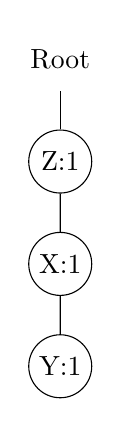
\begin{tikzpicture}[every node/.style={circle,draw,minimum size=0.8cm, inner sep=1pt}, level distance=1.3cm]
      \node[rectangle, draw=none] {Root}
        child {node {Z:1}
          child {node {X:1}
            child {node {Y:1}}
          }
        };
    \end{tikzpicture}
    \end{center}

    \vspace{1.5em}
    \textbf{2) FP-Tree after inserting $T_5$}
    \begin{center}
    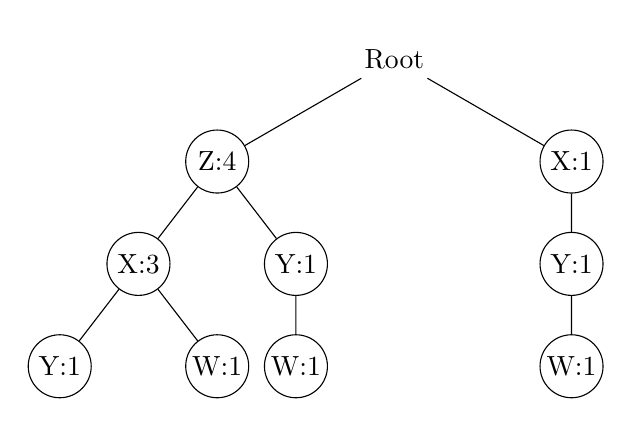
\begin{tikzpicture}[every node/.style={circle,draw,minimum size=0.8cm, inner sep=1pt}, level distance=1.3cm, level 1/.style={sibling distance=4.5cm}, level 2/.style={sibling distance=2cm}]
      \node[rectangle, draw=none] {Root}
        child {node {Z:4}
          child {node {X:3}
            child {node {Y:1}}
            child {node {W:1}}
          }
          child {node {Y:1}
            child {node {W:1}}
          }
        }
        child {node {X:1}
          child {node {Y:1}
            child {node {W:1}}
          }
        };
    \end{tikzpicture}
    \end{center}

    \vspace{1.5em}
    \textbf{3) Final FP-Tree after inserting $T_8$}
    \begin{center}
    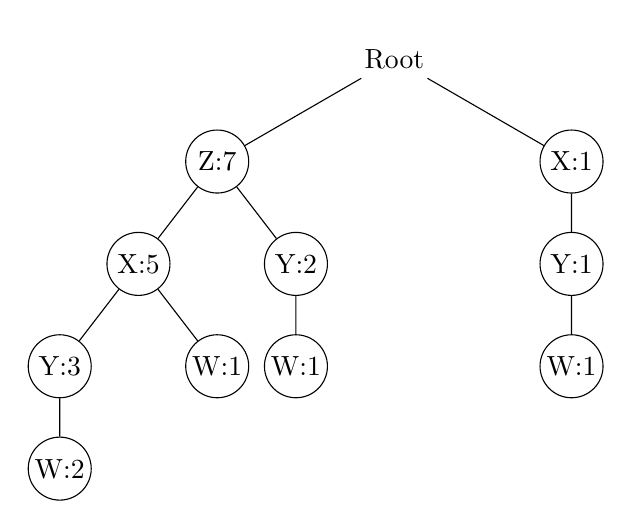
\begin{tikzpicture}[every node/.style={circle,draw,minimum size=0.8cm, inner sep=1pt}, level distance=1.3cm, level 1/.style={sibling distance=4.5cm}, level 2/.style={sibling distance=2cm}]
      \node[rectangle, draw=none] {Root}
        child {node {Z:7}
          child {node {X:5}
            child {node {Y:3}
              child {node {W:2}}
            }
            child {node {W:1}}
          }
          child {node {Y:2}
            child {node {W:1}}
          }
        }
        child {node {X:1}
          child {node {Y:1}
            child {node {W:1}}
          }
        };
    \end{tikzpicture}
    \end{center}
    
    
\end{enumerate}

\newpage
% ==========================================
% Question 2
% ==========================================
\section*{2. Sequential Pattern Mining (25 points)}

\begin{enumerate}[label=(\alph*)]
    \item
    The length-1 frequent sequential patterns and their absolute supports are:
    \begin{itemize}
        \item $\langle a \rangle$: 4 (in T1, T2, T3, T6)
        \item $\langle b \rangle$: 3 (in T1, T3, T6)
        \item $\langle c \rangle$: 5 (in T1, T2, T3, T4, T6)
        \item $\langle d \rangle$: 3 (in T1, T3, T5)
        \item $\langle e \rangle$: 2 (in T2, T4)
        \item $\langle g \rangle$: 2 (in T1, T5)
    \end{itemize}    
    \vspace{2em}
    
    \item
    The projected database for prefix $\langle(ab)\rangle$ consists of the suffixes of sequences containing $\langle(ab)\rangle$:
    \begin{itemize}
        \item T1: $\langle bc(dg) \rangle$
        \item T3: $\langle (cd) \rangle$
        \item T6: $\langle bc \rangle$
    \end{itemize}
    Yes, the support of $\langle(ab)\rangle$ is \textbf{3}.
    
    \vspace{2em}
    
    \item
    The prefix $\langle ab \rangle$ indicates item $a$ is followed by item $b$ in a separate subsequent itemset. The projected database is derived by finding the first instance of $a$, and then the first instance of a new subsequent itemset containing $b$:
    \begin{itemize}
        \item T1: $\langle c(dg) \rangle$
        \item T6: $\langle c \rangle$
    \end{itemize}
    Yes, the support of $\langle ab \rangle$ is \textbf{2}.
    
    \vspace{2em}
    
    \item
    The projected database for prefix $\langle a \rangle$ is obtained by finding the first occurrence of $a$ and taking the suffix. We use the conventional notation $\_b$ to indicate that $b$ is in the same itemset as the matched prefix item $a$.
    \begin{itemize}
        \item T1: $\langle (\_b)bc(dg) \rangle$
        \item T2: $\langle (ce)eh \rangle$
        \item T3: $\langle (\_b)(cd) \rangle$
        \item T6: $\langle (\_b)bc \rangle$
    \end{itemize}
    
    \vspace{2em}
    
    \item
    By recursively mining the $\langle a \rangle$-projected database from 2(d), the frequent subsequences (support $\ge 2$) starting with $a$ in lexicographically increasing order are:
    \begin{enumerate}
        \item $\langle a \rangle$
        \item $\langle (ab) \rangle$
        \item $\langle (ab)b \rangle$
        \item $\langle (ab)bc \rangle$
        \item $\langle (ab)c \rangle$
        \item $\langle (ab)d \rangle$
        \item $\langle ab \rangle$
        \item $\langle abc \rangle$
        \item $\langle ac \rangle$
        \item $\langle ad \rangle$
    \end{enumerate}
    
    
\end{enumerate}

\newpage
% ==========================================
% Question 3
% ==========================================
\section*{3. Constraint-Based Pattern Mining (25 points)}

\begin{enumerate}[label=(\alph*)]
    \item \textbf{(10 points) Given a collection of constraints (based on the Product table), identify their types (monotone, anti-monotone, data anti-monotone, succinct, convertible). If multiple types coexist in the following constraints, please list them all.}
    \begin{enumerate}[label=\roman*.]
        \item \textbf{(3 points) Total price of all purchased items is less than \$250.}
        \\
        % TODO: Answer here.
        
        
        \vspace{1em}
        \item \textbf{(3 points) Total price of all purchased items is at least \$200.}
        \\
        % TODO: Answer here.
        
        
        \vspace{1em}
        \item \textbf{(4 points) The minimal price of the purchased item is less than \$50.}
        \\
        % TODO: Answer here.
        
        
    \end{enumerate}

    \vspace{2em}
    
    \item \textbf{(10 points) Constraints are important pieces of information that may speed up frequent itemset mining.}
    \begin{enumerate}[label=\roman*.]
        \item \textbf{(3 points) What is a convertible constraint?}
        \\
        % TODO: Answer here.
        
        
        \vspace{1em}
        \item \textbf{(3 points) Give an example of a convertible constraint and explain how it can be pushed deep into the frequent itemset mining process to speed up mining.}
        \\
        % TODO: Answer here.
        
        
        \vspace{1em}
        \item \textbf{(4 points) Can your above constraint be pushed deep into the mining using the Apriori algorithm or it is confined to the pattern growth process (such as FP-Growth)? Briefly present your reasoning.}
        \\
        % TODO: Answer here.
        
        
    \end{enumerate}

    \vspace{2em}

    \item \textbf{(5 points) Let $A$ be an itemset (the pattern we are considering) and $V$ be a fixed bigger itemset. Is $A \subset V$ anti-monotone? If true, please explain the reason. Otherwise, please provide a counterexample.}
    \\
    % TODO: Answer here.
    
    
\end{enumerate}

\newpage
% ==========================================
% Question 4
% ==========================================
\section*{4. Null Invariance (25 points)}

\begin{enumerate}[label=(\alph*)]
    \item \textbf{(10 points) Suppose the following table shows two transaction data sets, $S_1$ and $S_2$, with the following count distributions after mining frequent 2-itemsets...}
    \begin{enumerate}[label=\roman*.]
        \item \textbf{(5 points) For each data set $S_1$ and $S_2$, compute support, confidence and lift for the following rules: $m \rightarrow c$ and $c \rightarrow m$.}
        \\
        % TODO: Compute metrics here.
        
        
        \vspace{1em}
        \item \textbf{(5 points) Is lift a good correlation measure here? Why or why not? (Give one-line brief reasoning)}
        \\
        % TODO: Answer here.
        
        
    \end{enumerate}
    
    \vspace{2em}
    
    \item \textbf{(5 points) The definitions of two measures on frequent patterns, lift and cosine, look rather similar as shown below. Explain why one of these two measures is null-invariant but the other is not.}
    \\
    % TODO: Explain null-invariance difference.
    
    
    \vspace{2em}

    \item \textbf{(5 points) We have learned at least three correlation measures: (1) lift, (2) $\chi^2$, and (3) Kulczynski. Give one example for Kulczynski measure that it is the most appropriate measure among the three and explain why.}
    \\
    % TODO: Answer here.
    
    
    \vspace{2em}

    \item \textbf{(5 points) Explain: If null transactions are predominant in large datasets, Kulczynski and Imbalance Ratio are usually used together to measure the interestingness of a pattern.}
    \\
    % TODO: Answer here.
    
    
\end{enumerate}

\end{document}